% Gerado automaticamente. No preambulo do documento use:
% \usepackage{pgfplots}
% \pgfplotsset{compat=1.18}
\definecolor{plotblue}{HTML}{2563EB}
\definecolor{plotorange}{HTML}{D97706}
\definecolor{plotgreen}{HTML}{059669}
\definecolor{plotpurple}{HTML}{7C3AED}
\definecolor{plotgray}{HTML}{374151}
\definecolor{plotred}{HTML}{DC2626}
\definecolor{plotteal}{HTML}{0F766E}
\definecolor{plotslate}{HTML}{64748B}

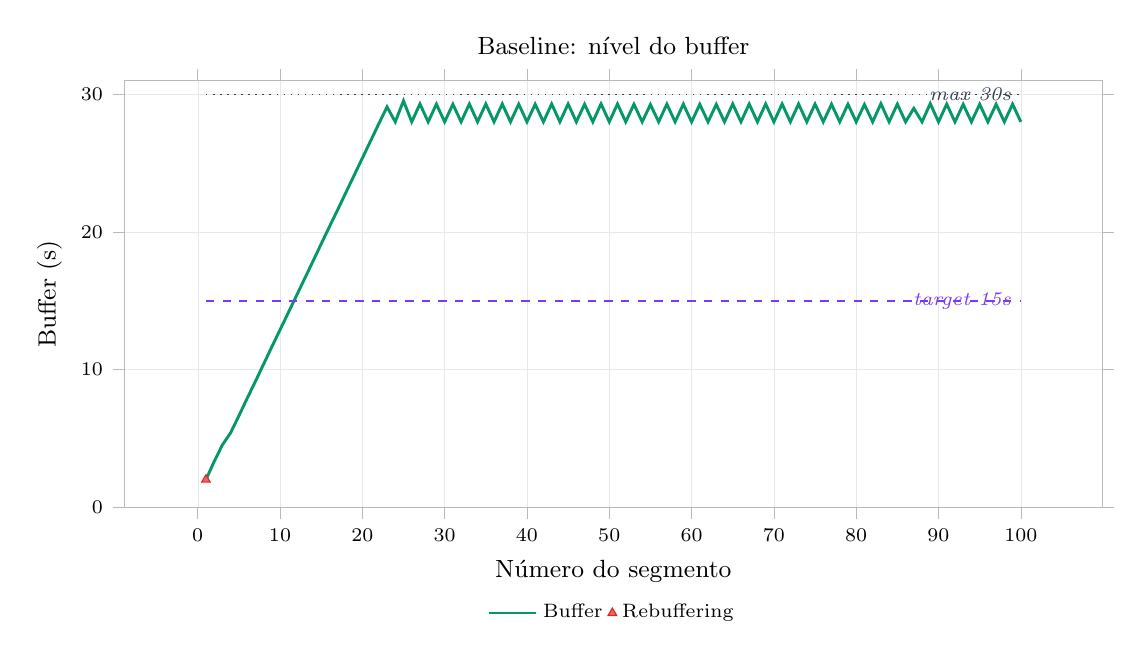
\begin{tikzpicture}
\begin{axis}[
    title={Baseline: nível do buffer},
    xlabel={Número do segmento},
    ylabel={Buffer (s)},
    width=14cm,
    height=7cm,
    grid=major,
    grid style={line width=.12pt, draw=gray!18},
    axis line style={draw=gray!55},
    tick style={draw=gray!55},
    tick align=outside,
    title style={font=\small},
    label style={font=\small},
    tick label style={font=\scriptsize},
    legend cell align={left},
    legend style={at={(0.5,-0.20)}, anchor=north, legend columns=3, draw=none, font=\scriptsize},
    ymin=0,
    ymax=31
]
\addplot+[plotgreen, line width=1.05pt, mark=none] coordinates {
(1,2)
(2,3.32)
(3,4.53)
(4,5.41)
(5,6.64)
(6,7.9)
(7,9.13)
(8,10.39)
(9,11.65)
(10,12.89)
(11,14.13)
(12,15.37)
(13,16.62)
(14,17.87)
(15,19.13)
(16,20.38)
(17,21.61)
(18,22.86)
(19,24.11)
(20,25.36)
(21,26.61)
(22,27.86)
(23,29.09)
(24,28)
(25,29.53)
(26,28)
(27,29.3)
(28,28)
(29,29.29)
(30,28)
(31,29.28)
(32,28)
(33,29.3)
(34,28)
(35,29.3)
(36,28)
(37,29.3)
(38,28)
(39,29.29)
(40,28)
(41,29.28)
(42,28)
(43,29.3)
(44,28)
(45,29.3)
(46,28)
(47,29.28)
(48,28)
(49,29.31)
(50,28)
(51,29.3)
(52,28)
(53,29.28)
(54,28)
(55,29.26)
(56,28)
(57,29.29)
(58,28)
(59,29.29)
(60,28)
(61,29.27)
(62,28)
(63,29.27)
(64,28)
(65,29.3)
(66,28)
(67,29.3)
(68,28)
(69,29.3)
(70,28)
(71,29.3)
(72,28)
(73,29.3)
(74,28)
(75,29.29)
(76,28)
(77,29.28)
(78,28)
(79,29.28)
(80,28)
(81,29.26)
(82,28)
(83,29.32)
(84,28)
(85,29.29)
(86,28)
(87,28.98)
(88,28)
(89,29.33)
(90,28)
(91,29.29)
(92,28)
(93,29.27)
(94,28)
(95,29.28)
(96,28)
(97,29.28)
(98,28)
(99,29.29)
(100,28)
};
\addlegendentry{Buffer}
\addplot+[plotpurple, dashed, line width=0.55pt, mark=none, forget plot] coordinates {(1,15) (100,15)};
\node[anchor=east, plotpurple, font=\scriptsize\itshape] at (axis cs:100,15) {target 15s};
\addplot+[plotgray, dotted, line width=0.55pt, mark=none, forget plot] coordinates {(1,30) (100,30)};
\node[anchor=east, plotgray, font=\scriptsize\itshape] at (axis cs:100,30) {max 30s};
\addplot+[only marks, mark=triangle*, mark size=1.8pt, plotred, mark options={solid, fill=plotred!70, draw=plotred}] coordinates {
(1,2)
};
\addlegendentry{Rebuffering}
\end{axis}
\end{tikzpicture}
